\section{An exact computation}\label{sec:computation}

To see sizes, we computed the bounded mixture of a small machine exactly. \emph{BF8} has eight commands,
coded by three input bits each and read from the input only when they are first needed:
\texttt{+} and \texttt{-} change the current cell by one modulo 16, \texttt{>} and \texttt{<} move along an
unbounded tape of cells, \texttt{[} jumps past the matching \texttt{]} if the cell is $0$, \texttt{]} jumps
back to just after the matching \texttt{[} if the cell is not $0$, and to the first command if there is no
matching \texttt{[}; \texttt{.}~prints the cell modulo 2 and \texttt{:} prints whether the cell is nonzero.
Each executed command is one step. A forward jump reads the commands it skips; they count as read and cost no
step. The mixture is that of \cref{def:mixture} with at most $10$ commands read ($L=30$ bits) and schedule
$T(k)=T_1k$. All masses are dyadic rationals and are computed without rounding by an enumerator that forks the
machine at every read ($8.6\cdot10^8$ branches for $T_1=24$; $8.4\cdot10^5$ strings of length at most 48 have
positive mass). The enumerator agrees with a run of all command tapes for small $L$.

BF8 is not universal in the sense of \cref{def:universal}, since a program cannot read the rest of its input
as data, and one of its steps can read several commands. So \cref{thm:twin,thm:quine,thm:search,thm:capture,thm:machine}
do not apply to it as stated, and it has no wrappers. \Cref{lem:basic,thm:calibration,thm:budget,thm:feedback,thm:contrarian}
hold for every machine. The computation concerns prediction only.

For a stream $z$ and a position $k$ we report three shares of the posterior given $z_{1:k-1}$: the mass that
prints the true bit $z_k$ on schedule (``true''), the mass that prints the other bit (``other''), and the rest
(``none''), which prints nothing on schedule or would need an eleventh command first. \Cref{tab:profiles}
gives selected positions, and \cref{fig:profiles} the full profiles.

\begin{table}[ht]\centering\small
\begin{tabular}{lr@{\qquad}rrr@{\qquad}rrr}
\toprule
 & & \multicolumn{3}{c}{$T(k)=24k$\qquad\mbox{}} & \multicolumn{3}{c}{$T(k)=3k$} \\
stream & $k$ & true & other & none & true & other & none \\
\midrule
$1^{48}$ & 16 & 0.791 & 0.205 & 0.004 & 0.544 & 0.451 & 0.005 \\
$1^{48}$ & 31 & 0.963 & 0.037 & 0.001 & 0.869 & 0.130 & 0.001 \\
$(10)^{24}$ & 17 & 0.294 & 0.457 & 0.249 & 0.141 & 0.411 & 0.448 \\
$(10)^{24}$ & 31 & 0.935 & 0.062 & 0.003 & 0.842 & 0.155 & 0.003 \\
$0^{48}$ & 17 & 0.958 & 0.008 & 0.034 & 0.969 & 0.012 & 0.019 \\
$1^80^{40}$ & 9 & 0.025 & 0.958 & 0.017 & 0.001 & 0.998 & 0.001 \\
\bottomrule
\end{tabular}

\caption{Posterior shares at selected positions, BF8 with at most 10 commands. Exact values rounded to three
places.}\label{tab:profiles}
\end{table}

\begin{figure}[ht]\centering
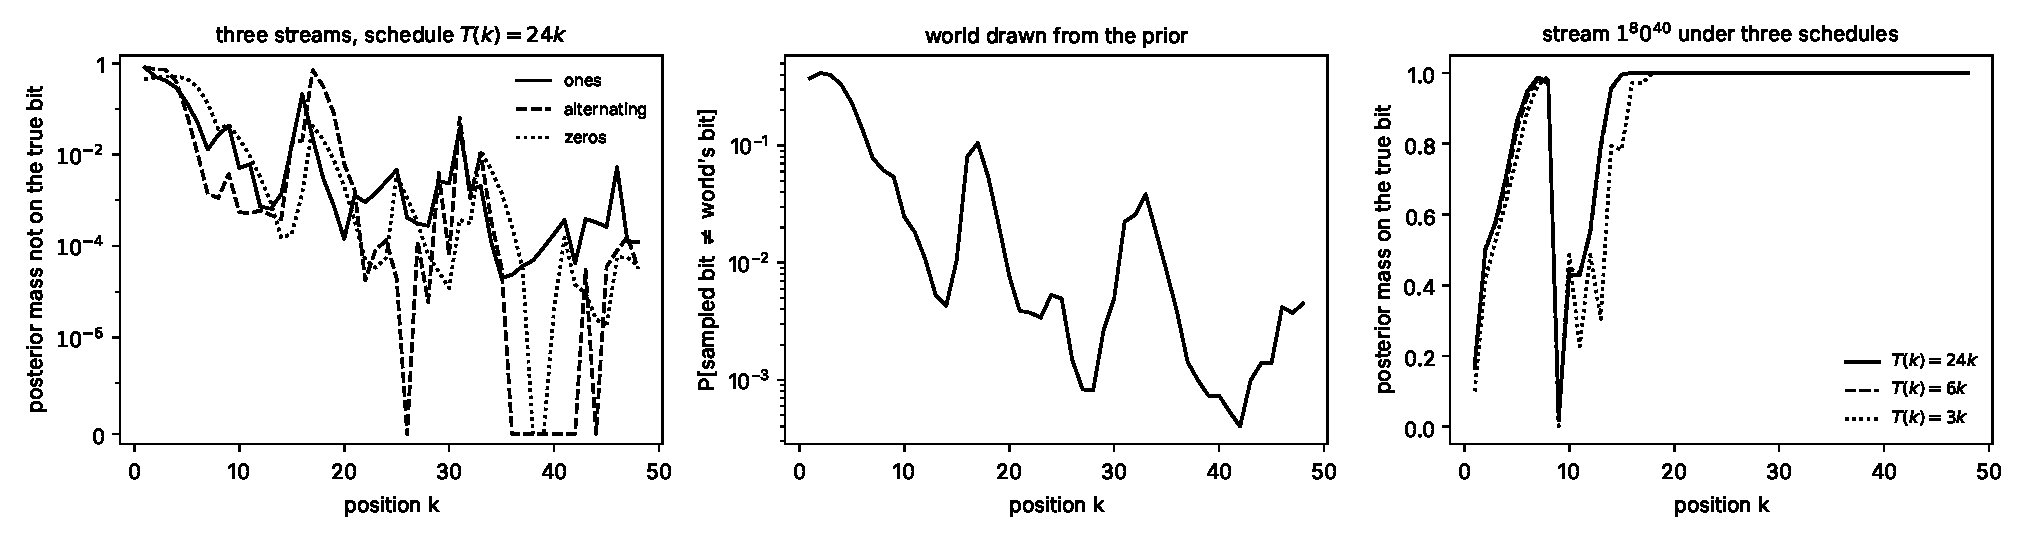
\includegraphics[width=\textwidth]{../experiments/results/profiles.pdf}
\caption{Left: posterior mass not on the true bit, by position, for three streams (the axis is linear near
$0$, so exact zeros are visible). Middle: probability that the sampled next bit differs from the world's own,
for a world drawn from the prior that prints that bit within the bounds (by \cref{thm:calibration} both bits
are independent draws from the predictor's distribution). Right: mass on the true bit for the stream
$1^80^{40}$ under three schedules.}\label{fig:profiles}
\end{figure}

\paragraph{A shorter program explains the context and continues differently.} Both large effects in
\cref{tab:profiles} have this cause, and in both the short programs use the rule that an unmatched \texttt{]}
restarts the program while the cell is nonzero, together with the fact that a cell returns to $0$ after
sixteen increments.
\begin{itemize}[leftmargin=1.4em,itemsep=1pt,topsep=2pt]
\item The stream $1^{48}$ is printed forever by four-command programs such as \texttt{+[:]}, and by no shorter
one. The three-command programs \texttt{+:]} and \texttt{-:]} print $1^{15}0$ and then run on into whatever
commands follow. They carry $2\cdot8^{-3}$ of the mass $0.00554$ on $1^{15}0$, which is $70\%$. At bit 16 a
share $0.205$ of the posterior prints the other bit, and at bit 31 a share $0.037$. From position 10 on, the
mass off the true bit is below $0.01$ everywhere except at positions 15--17 and 31.
\item The alternating stream is printed forever by six-command programs such as \texttt{++[:.]}, and by no
shorter one. The three-command programs \texttt{+.]} and \texttt{-.]} print its first 16 bits and then run on.
They carry $2\cdot8^{-3}$ of the mass $0.00682$ on these 16 bits, which is $57\%$. At bit 17 the true bit has
share $0.294$, the other bit $0.457$, and $0.249$ is in ``none''; normalised over the two bits, the true one
has $0.392$. So the majority form of \cref{def:mph} holds for this world at this cut point, for the predictor
with at most ten commands.
\end{itemize}
This is the first sentence of \cref{sec:capture} in action: the programs for the context that do not continue
with the world's own bit outweigh those that do. Nothing here acts for a purpose. The example shows only that
the inequality can go the wrong way at an exactly computable place, and that a stopping point which is cheap
on the machine, here the return of a counter to zero, is where it does.

\paragraph{The effect weakens as longer programs are admitted.} \Cref{tab:length} repeats the computation
with at most 7 to 11 commands. The mass that continues with the true bit is spread over many program lengths
and keeps growing with the bound, while the mass of the short programs that leave is counted in full from the
start. At bit 17 of the alternating stream the normalised share of the true bit rises from $0.273$ to $0.416$,
and part of ``none'' at the smaller bounds is mass cut off by the bound itself. We did not compute beyond 11
commands, so whether the majority at bit 17 persists for much longer programs is not known from this
computation.

\begin{table}[ht]\centering\small
\begin{tabular}{rrrrrr}
\toprule
 & \multicolumn{4}{c}{bit 17 of $(10)^{24}$} & bit 16 of $1^{48}$ \\
commands & true & other & none & true, normalised & other \\
\midrule
7 & 0.157 & 0.419 & 0.424 & 0.273 & 0.275 \\
8 & 0.210 & 0.442 & 0.348 & 0.322 & 0.243 \\
9 & 0.256 & 0.452 & 0.291 & 0.362 & 0.221 \\
10 & 0.294 & 0.457 & 0.249 & 0.392 & 0.205 \\
11 & 0.326 & 0.458 & 0.217 & 0.416 & 0.194 \\
\bottomrule
\end{tabular}

\caption{The two headline positions under different bounds on the number of commands, $T(k)=24k$.}\label{tab:length}
\end{table}

\paragraph{The budget holds with room.} \Cref{tab:budget} compares both sides of the finite forms of
\cref{thm:budget}(ii) and (iii) for the first 48 bits.

\begin{table}[ht]\centering\small
\begin{tabular}{lrrrr}
\toprule
stream & $\sum_{k\le48}(1-\mathrm{true}_k)$ & $\ln(1/\xi(z_{1:48}))$ & $\#\{k:\mathrm{true}_k\le\frac12\}$ & $\log_2(1/\xi(z_{1:48}))$ \\
\midrule
$1^{48}$ & 2.63 & 3.94 & 2 & 5.68 \\
$0^{48}$ & 3.07 & 4.03 & 2 & 5.82 \\
$(10)^{24}$ & 4.01 & 6.76 & 4 & 9.76 \\
$1^80^{40}$ & 5.07 & 9.77 & 5 & 14.09 \\
\bottomrule
\end{tabular}

\caption{The budget inequalities for $T(k)=24k$ and at most 10 commands, with $\xi(z_{1:48})$ in place of the
limit: ``true$_k$'' is $\xi(z_k\mid z_{1:k-1})$.}\label{tab:budget}
\end{table}

\paragraph{The population.} For a world drawn from the prior that prints the bit in question within the
bounds, the probability that a sampled next bit differs from the world's own is $0.080$, $0.105$, $0.054$ at
positions 16, 17, 18 and between $0.022$ and $0.038$ at positions 31--33; its median over positions 20--28 and
36--44 is $0.0014$ (\cref{fig:profiles}, middle). By \cref{thm:calibration} this is neither more nor less than
the unpredictability of such worlds at these positions.

\paragraph{A tighter schedule can shift mass off the truth.} With $T(k)=3k$ in place of $24k$, the share of
the true bit falls from $0.791$ to $0.544$ at bit 16 of $1^{48}$, from $0.294$ to $0.141$ at bit 17 of the
alternating stream, and from $0.025$ to $0.001$ at bit 9 of $1^80^{40}$ (\cref{tab:profiles}). The shift is
not uniform: at bit 17 of $0^{48}$ the share rises from $0.958$ to $0.969$. With at most nine commands the
stream $1^80^{40}$ shows the extreme case of \cref{sec:time}: under $T(k)=24k$ it has mass $1593\cdot2^{-25}$
on all 48 bits, while under $T(k)=3k$ its first 14 bits have mass $2^{-26}$, the true 15th bit has mass $0$
and the other bit $2^{-26}$. The tight predictor gives the truth probability $0$ there, and all of its
posterior to a continuation the world does not have.
